% !TeX root = ../../../main.tex

%************************************************
\section{Positivity of partonic cross sections}
\label{sec:pos/subtr}
%************************************************

QCD factorization allows expressing physical cross sections $\sigma$  as
convolutions of partonic cross sections with parton distributions $f_i$. 
In the prototypical case of DIS the cross section is expressed in terms of
hadronic structure functions $F(x,Q^2)$, which are then factorized in terms of
parton-level structure functions, called coefficient functions $C_i$:
\begin{equation}
  \label{eq:masterfac}
 \frac{1}{x} F(x,Q^2)=\sum_{i} e^2_i C_i \otimes f_i ,
\end{equation}
where the sum runs over all parton species, $e_i$ are quark electric charges,
or the sum over all electric charges for the gluon, (for photon-induced DIS,
and more in general electroweak charges), $\otimes$ denotes convolution, and we
refer to Ref.~\cite{Ellis:1991qj} for notations and conventions. 
The convolution in Eq.~(\ref{eq:masterfac}) links the three a priori physically
distinct scaling variables on which respectively the physical observable $F$,
the partonic cross-section $C$ and the PDF $f$ depend.
In the sequel, for
clarity, we will denote with $x$ the physically observable variable
(Bjorken-$x$ for DIS, or the scaling variable in hadronic collisions), with $z$
the variable on which the coefficient function depends, and with $\xi$ the PDF
momentum fraction.
Of course, Mellin transformation turns the convolution into an ordinary product
and upon transformation all these variables are mapped onto the same $N$
variable. 
 

  At LO all factors on the
  right-hand side of
  Eq.~(\ref{eq:masterfac}) are manifestly positive. Indeed, the partonic
  cross sections (which for DIS at LO are trivial) are defined as the square modulus of amplitudes. The
  PDFs in turn are defined as operator matrix elements
  which can be interpreted as probability
  distributions~\cite{Collins:1981uw,Curci:1980uw}: for quark
  PDFs~\cite{Collins:1981uw}  
  \begin{equation}
    \label{eq:quark}
f_i(\xi)=\frac{1}{4\pi}\int dy^- e^{-i \xi P^+ y^-}\langle P| 
\bar \psi_i(0,y^-,\vec 0_T)\gamma^+ {\cal P} \exp\left[ i g_s \int_0^{y^-} d
  \bar y^- A_a^+(0,\bar y^-,\vec 0_T)\frac{1}{2} \lambda_a\right] \psi_i(0) |P\rangle ,
\end{equation}
where ${\cal P}$ denotes path-ordering; $P$ is the four-momentum of
the parent hadron in light-cone components and $g_s$ is the strong
coupling, with analogous expressions for antiquarks and
gluons~\cite{Collins:1981uw}.  It can be shown (see
e.g.\ Sect.~6.7 of Ref.~\cite{Collins:2011zzd}) that the expression
Eq.~(\ref{eq:quark}) is a number density, and as such before
subtraction of divergences it is positive.

Beyond LO, besides ultraviolet renormalization, both the
PDFs and the partonic cross section are beset by collinear
singularities which can be factored into the PDF. Before
factorization the PDF is a ``bare'' probability density $f_i^{(0)}$~\cite{Collins:2011zzd}, while after
factorization it is a
renormalized PDF  $f_i$
\begin{equation}
  \label{eq:pdffac}
f_i =\sum_{j} Z^S_{ij}\otimes f_j^{(0)}. %\cr
\end{equation}
In operator language, the  factor $Z^S_{ij}$ is a multiplicative
renormalization of the operator Eq.~(\ref{eq:quark}), which admits a
perturbative expansion
\begin{equation}\label{eq:pertz}
Z^S_{ij}(Q^2)=\delta_{ij}+\frac{\alpha_s}{2\pi}
\delta^S_{ij}(Q^2)+O(\alpha_s^2),
\end{equation}
where $\delta^S_{ij}$ is a counterterm which diverges after
regularization is removed, the superscript $S$ denotes the fact
that the finite part of the counterterm depends on the choice of a
particular subtraction scheme $S$, and regularization induces a
dependence of the counterterm and thus of the renormalization constant
on scale.

The counterterm can be determined
in a standard way by taking the matrix element of the
operator in a state in which the right-hand side of
Eq.~(\ref{eq:quark}) is perturbatively computable, such as a free
state of a parton $i$, in which the PDF for finding a parton $j$ is
trivially
\begin{equation} \label{eq:freef}
  f_j^{i\,(0)}(\xi)=\delta_{ij}\delta(1-\xi),
\end{equation}
imposing a
renormalization condition and finally removing the regulator. In practice, this
is most easily done~\cite{Collins:2011zzd,Curci:1980uw} by introducing
a probe that couples to the free 
quark, so for instance computing the structure function
Eq.~(\ref{eq:masterfac}) for deep-inelastic scattering off a free
quark. This is the strategy that we will follow in this section, where
such a computation will be performed explicitly in a way that fully
determines the factorization scheme, both in the \msbar{} and in our
new positive schemes.


The factorization argument then works as follows. The $d$-dimensional structure
function Eq.~(\ref{eq:masterfac}) is
written as
\begin{align} \label{eq:refaca}
 \frac{1}{x} F_i(x,Q^2,\epsilon)&=\sum_{j} e^2_j C_j \otimes f_j^{i\,(0)} \\
&=\sum_{j} e^2_j C_j^S \otimes f_j^{i\,S};\qquad\quad d=4-2\epsilon,
\label{eq:refacb}
\end{align}
and computed by taking in turn  the incoming parton to be each of the
parton species, i.e. using Eq.~(\ref{eq:freef}).
  Of course, the structure
function on the l.h.s.\ then reduces to the
unsubtracted, regularized coefficient
function, which is essentially the cross-section for scattering off
the given incoming free parton. The counterterm is defined by imposing the
cancellation of the singularity. Up to NLO, assuming a free incoming
parton according to Eq.~(\ref{eq:freef}), substituting in
Eqs.~(\ref{eq:refaca}-\ref{eq:refacb}) the
perturbative expression Eq.~(\ref{eq:pertz}) of the 
renormalization factor Eq.~(\ref{eq:pdffac}), and assuming a
perturbative expansion of the coefficient functions of the form
\begin{equation}\label{eq:perc}
  C_i(z,Q^2)= C^{(0)}_i(z,Q^2)+\frac{\alpha_s}{2\pi} C^{(1)}_i(z,Q^2)+O(\alpha_s^2)
\end{equation} 
one gets
\begin{equation}\label{eq:renorm}
    C_i^S(z,Q^2,\epsilon) = 
    {C^{(1)}_{i}}(z,Q^2,\epsilon)
    -\delta_{qi}^S(z,Q^2,\epsilon)\,,
\end{equation}
where $q$ denotes a quark parton.
Note that, up to NLO, imposing finiteness of the DIS structure
functions fixes the renormalization in the quark sector because DIS is
a probe that only couples to quarks at leading order.

The advantage of determining the counterterms in this way, as opposed
to performing a direct computation of the current matrix element
Eq.~(\ref{eq:quark}) is that in  operator matrix
elements all divergences appear as ultraviolet, while, when computing a
structure function for an incoming free parton  (or, more
generally, a generic partonic cross-section), collinear singularities
come from the infrared region of integration over
transverse momenta. Hence, one may compute the relevant
cross-section using renormalized perturbation theory (i.e., with
counterterms already included in the Lagrangian). The only divergences
are then of collinear and infrared origin.
The regularized partonic cross-section is
then finite if the computation is
performed with $\epsilon<0$, and it enjoys the positivity
properties of a standard 
cross-section. This property will be crucial in the argument presented
 below.

After the subtraction Eq.~(\ref{eq:renorm}), the partonic cross-section
(coefficient function) is
finite in the $\epsilon\to0$ limit, so one may define the
four-dimensional coefficient function as
\begin{equation}\label{eq:crenorm}
    {C^{(1)}_{i}}^S(z) = \lim_{\epsilon\to0^-}\left( {C^{(1)}_{i}}(z,Q^2,\epsilon)
    -\delta_{qi}^S(z,Q^2,\epsilon)\right),
\end{equation}
where $\epsilon\to 0^-$ denotes the fact that the limit is taken from
below, as discussed above. Note that the four-dimensional coefficient
function function can depend only on $z$ for dimensional reasons,
while the $d$ dimensional one  also depends on $Q^2$ through the
combination $\frac{Q^2}{\mu^2}$, where $\mu^2$ is the scale of
dimensional regularization. That this subtraction is always possible
is the content of factorization
theorems~\cite{Collins:2011zzd,Curci:1980uw}. The universal
(i.e.\ process-independent) nature of the collinear singularities
ensure that the renormalization conditions on parton distributions,
defined as operator matrix elements Eq.~(\ref{eq:quark})
without reference to any specific
process, may be determined by the computation of a particular process
or set of processes as discussed here.

The finite part of the
subtraction is arbitrary and it defines the factorization scheme $S$. In
\msbar{} it turns out that in some partonic subchannels the
subtracted cross section can be negative:
effectively, negative finite parts are factored away from the
regularized cross sections, and into the PDFs. These can then
also become negative, though whether this happens or not depends on
the relative weight of the various subchannels.
On the other hand, the residue of
the collinear pole is universal---it is given by
process-independent splitting functions---and this makes it possible
to define its subtraction in a way that preserves positivity of the
partonic cross section at the regularized level. If all contributions
which are factored away from the partonic cross section and into the
PDF remain positive, then the latter also stays positive.


Having explained the general strategy, we now implement it
explicitly. 
We first discuss DIS structure functions.
We  then turn to hadronic processes, both quark-induced and gluon induced.


\subsection{Deep-inelastic coefficient functions}
\label{sec:discf}
At NLO, photon-induced DIS proceeds through the two
sub-processes $q+\gamma^*\to X$ and $g+\gamma^*\to X$, in such a way
that the contribution of each quark or antiquark flavor to the
structure function $F_2$ can be written as:
\begin{equation}\label{eq:f2}
 \frac{1}{x} F_2(x,Q^2)= e_q^2 \left[q
 +\frac{\alpha_s}{2\pi}\left( C^{(1)}_q \otimes q+ C^{(1)}_g \otimes
 g\right)\right](Q^2)\,,
 \end{equation}
where $e_q$ is the electric charge of the quark, on the right-hand
side we have omitted the $x$ dependence which arises from the
convolution,
and the
generalization to $Z$- and $W$-induced DIS is trivial.

\begin{figure}[t]
  \begin{center}
    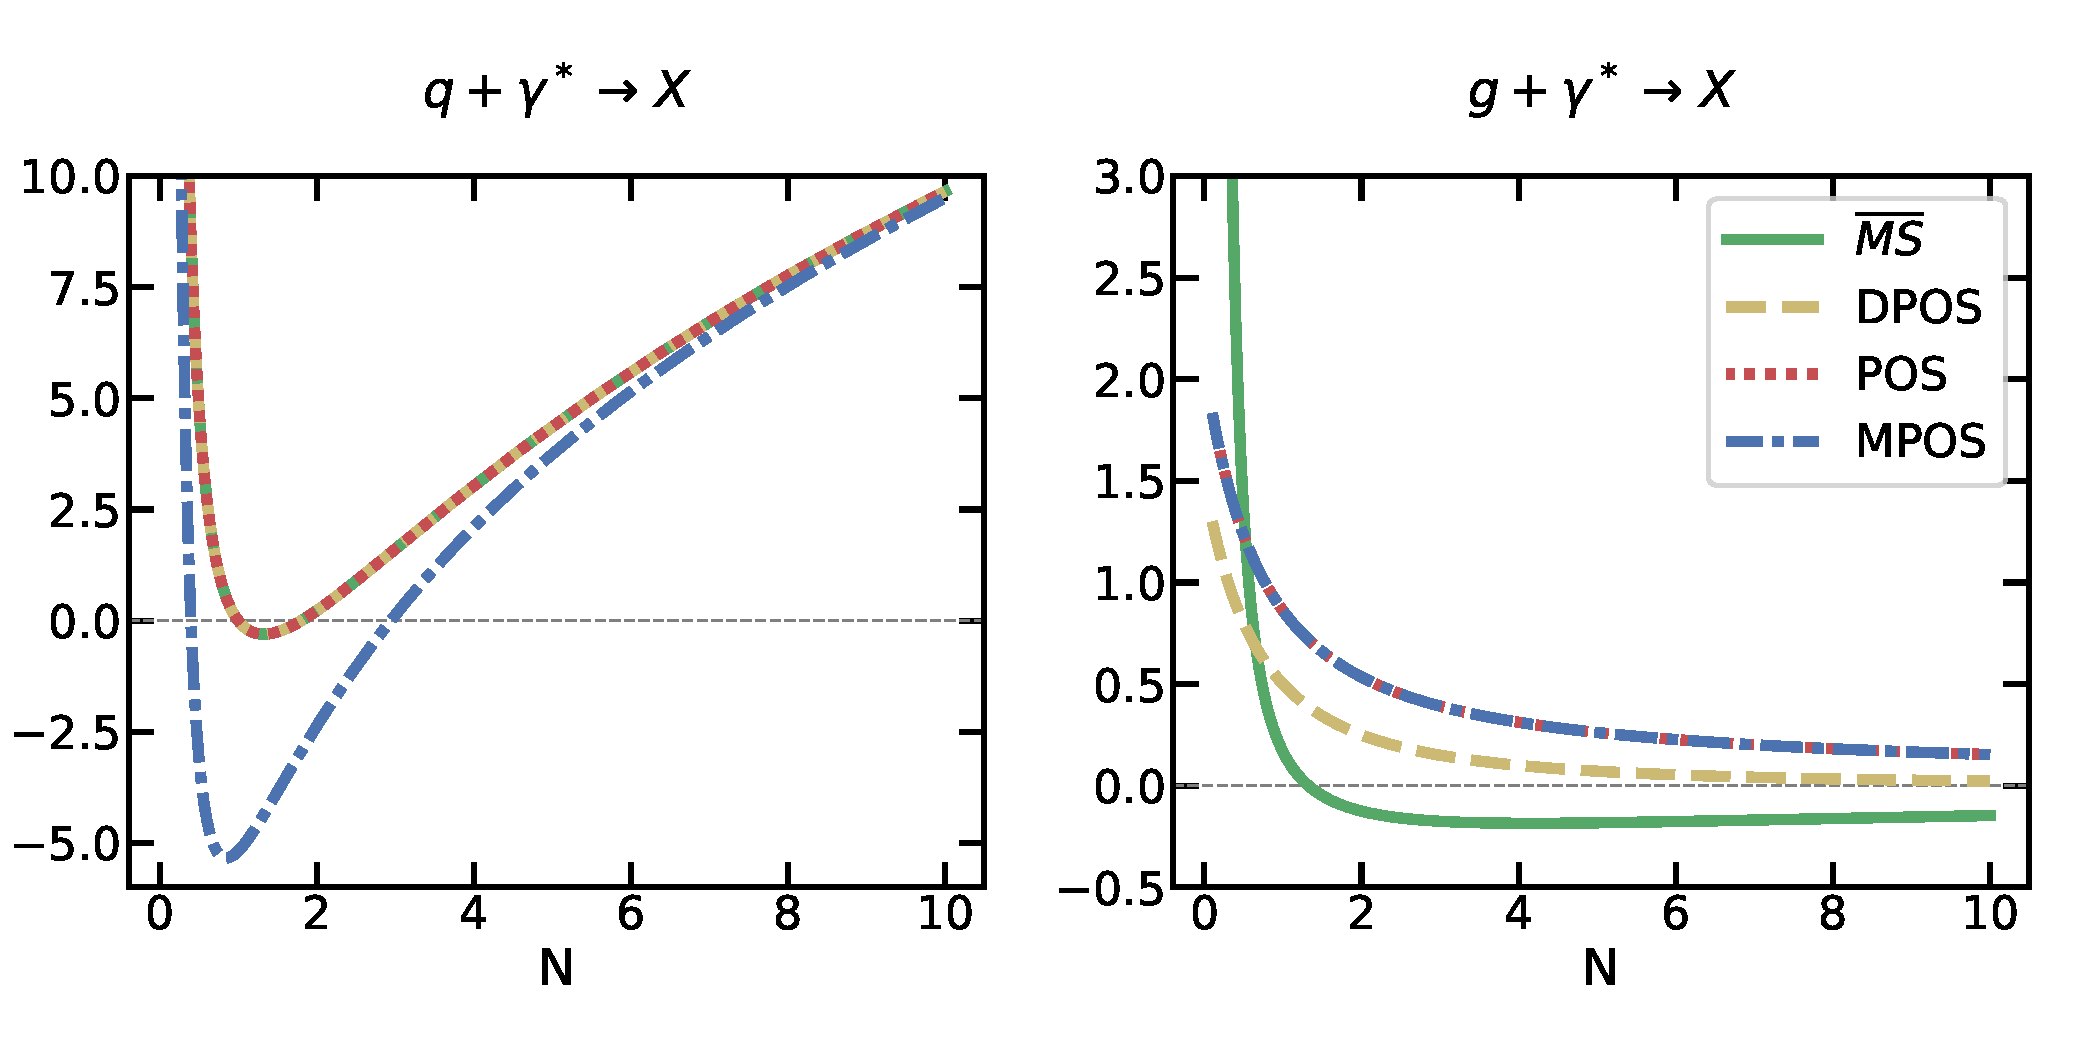
\includegraphics[width=0.8\linewidth]{ch-positivity/dis.pdf}
    \caption{\small Mellin-space NLO contributions to deep-inelastic coefficient
      functions. The quark (left) and gluon (right) coefficient
      functions, respectively $C_q^{(1)}$ and $C_g^{(1)}$, Eq.~\ref{eq:f2}, are
      shown. The DPOS
      scheme is defined in Eqs.~(\ref{eq:count},\ref{eq:countq}), the POS
      scheme is defined in Eqs.~(\ref{eq:counthqq}-\ref{eq:counthqg}),
      and the MPOS scheme
      in Eqs.~(\ref{eq:mposqq}-\ref{eq:mposqg}).
      Results are shown in the \msbar{} and DPOS, POS and MPOS
      schemes. For  $C_q^{(1)}$ \msbar{}, DPOS and POS
      coincide, and the two curves shown correspond, from top to
      bottom, to \msbar{} and MPOS; for $C_g^{(1)}$ POS and MPOS
      coincide and the three
      curves correspond,
      from  bottom to top, to \msbar{}, DPOS and POS.
    \label{fig:dis} }
  \end{center}
\end{figure}
  The
  \msbar{} NLO contributions to the coefficient functions
  $C_q$ and $C_g$ are shown in Fig.~\ref{fig:dis} in Mellin space,
  where the convolution becomes an ordinary product. The
  Mellin space plot is especially transparent since the $x$-space
  cross section is found to high accuracy by computing the inverse
  Mellin transform in the saddle-point
  approximation~\cite{Bonvini:2012an}: hence, the physical  $x$-space
  cross section is just the product of the Mellin-space coefficient
  function and PDF evaluated at the value of $N$ corresponding to the
  saddle for given kinematics. 
  It is clear  from Fig.~\ref{fig:dis} that at
  large $N$ the gluon coefficient function is negative on the real
  axis: hence, the $x$-space coefficient function must also be
  negative because its real moments are negative. This shows
 that a negative contribution has been factored from the coefficient
 function into the PDF. 


 
\subsubsection{Over-subtraction and the off-diagonal coefficient function}
\label{sec:offdiag}

In order to understand what is going on, we look at the dimensionally
regularized, unsubtracted gluon coefficient function:
\begin{equation}\label{eq:cgeps}
C^{(1)}_{g}(z,Q^2,\epsilon) = \frac{ \Gamma(-\epsilon)
  \left(\frac{\mu_D^2}{\pi\mu^2}\right)^{-\epsilon} \left[8P_{qg}(z)-16 T_R \epsilon (3
    -\epsilon(2 -\epsilon) )  \right]  }{16\pi (2 - 2\epsilon) \Gamma (3 - 2 \epsilon)}\,,
\end{equation}
where
\begin{equation}\label{eq:mud}
  \mu_D^2=\frac{s}{4}=\frac{Q^2(1-z)}{4z},
\end{equation} 
and  $s=\frac{Q^2(1-z)}{z}$ is the center-of-mass energy of the
$\gamma^* q$ collision. 
Note that in order to regulate the collinear singularity it is
necessary to choose $\epsilon<0$; it then follows that  as $\epsilon$
goes to zero from below,
$\Gamma(-\epsilon)>0$ and
the unsubtracted coefficient function, Eq.~(\ref{eq:cgeps}), is positive as it ought to
be.

The subtracted \msbar{} coefficient function is then given by
\begin{align}\label{eq:cgren}
{C^{(1)}_{g}}^{\mmsbar}(z) &= \lim_{\epsilon\to
  0^-}\left[C_{g}^{(1)}(z,Q^2,\epsilon) - \left(\frac{Q^2}{4\pi
      \mu^2}\right)^{-\epsilon} \left(-\frac 1
    {\epsilon}+\gamma_E\right) P_{qg}(z)\right]\\
    &= P_{qg}(z) \left( \ln\left(\frac{1-z}{z}\right) - 4 \right) + 3
    T_R \, ,\label{eq:cgnlo}
\end{align}
where  $\epsilon\to 0^-$ denotes the fact that the limit should be
taken from below, because the collinear singularity is regulated with
$\epsilon<0$. 
The $P_{qg}$ splitting function is positive for all $z$, so for
$z>\frac{1}{2}$ the log  becomes negative and at large $z$ the
coefficient function is negative.


Comparing  Eqs.~(\ref{eq:cgeps}-\ref{eq:cgren}) immediately reveals
what happened:  the regularized coefficient function contains a term
\begin{equation}\label{eq:logexp}
  \left(\frac{s/4}{\pi\mu^2}\right)^{-\epsilon}=1-\epsilon \ln \left(\frac{Q^2(1-z)/z}{4\pi\mu^2}\right),
\end{equation}
but in the collinear subtraction $\ln \frac{Q^2}{4\pi\mu^2}$ has been
subtracted instead. For $z>\frac{1}{2}$, $s<Q^2$ this
amounts to over-subtracting, at the larger scale $Q^2$ instead of the
smaller physical scale $s$. The physical origin of this contribution,
and the reason for the mismatch are easy to trace.

Namely, this is the
contribution coming from quark emission from the incoming gluon line,
and the singularity is due to the collinear singular integration over
the transverse momentum of the emitted quark, as revealed by the fact
that it is proportional to the corresponding $P_{qg}$ splitting
function. The argument of the ensuing collinear log is set by the
upper limit of the transverse momentum integration $k_T^{\textrm{max}}$,
which for a $2\to2$ process with massless particles in the final state
is $k_T^{\textrm{max}}=\frac{s}{4}$. In \msbar{}
the collinear subtraction is performed at the scale $Q^2$,
hence leading to the over-subtraction that we observed, and producing
a contribution to the coefficient function which is logarithmically
enhanced in the threshold $z\to1$ limit.

Therefore, this contribution has the same origin as the soft (Sudakov)
logarithms 
which are resummed to all orders
when performing threshold
resummation~\cite{Catani:1989ne,Sterman:1986aj}, except that 
in soft resummation the splitting function is evaluated in the $z\to1$
limit, and the factor of $\frac{1}{z}$ in the argument of the log is
neglected.
In fact, threshold resummation can be
obtained by identifying (and then
renormalization-group improving)
\begin{equation}\label{eq:ktmax}
 |k_T^{\textrm{max,\,DIS}}|^2=\mu_D^2
\end{equation}
(with $\mu_D^2$ given by Eq.~(\ref{eq:mud}))
  as the physical
scale in the soft limit~\cite{Forte:2002ni}. The over-subtraction is then
simply the manifestation of the well-known fact that, in the \msbar{} scheme,
threshold logs beyond the first are factored in the coefficient
function, and not in the PDF~\cite{Albino:2000cp}. Indeed, alternative
factorization schemes in which these logs are instead included in the
PDF have been proposed, in particular  the Monte Carlo
factorization scheme of Ref.~\cite{Jadach:2016acv}. Note, however, that
radiation in off-diagonal parton channels is power-suppressed in the
threshold limit, and indeed this contribution is proportional to
$\ln(1-z)$, which in Mellin space behaves as $\frac{\ln N}{N}$. This is to be
contrasted with the $\left(\frac{\ln(1-z)}{1-z}\right)_+$ behavior, corresponding to 
$\ln^2 N$, found in diagonal channels, as we shall discuss in
Sect.~\ref{sec:diag} below. Hence, while it has the same origin, this
contribution is not among those included in standard leading-power
threshold resummation. 

In conclusion,  in order to
restore positivity it is  sufficient to perform the collinear
subtraction at the scale $\mu_D^2=s/4$, Eq.~(\ref{eq:ktmax}).
There is a further subtlety, however. Namely, the factor $2-2\epsilon$
in the denominator of Eq.~(\ref{eq:cgeps}) is the average over the
polarization states of the incoming gluon. Therefore, it should be
viewed as an overall prefactor which is common to both the
unsubtracted and subtracted coefficient function, and thus  must be
included in the subtraction term. Because it interferes with a
$-\frac{1}{\epsilon}$ pole, not including it, as in \msbar{}, leads to
over-subtraction: 
the collinear singularity is regulated with
$\epsilon<0$, so $\frac{1}{1-\epsilon}<1$.  

Therefore, we define a modified positivity subtraction as
\begin{align}\label{eq:cgrenpos}
  {C^{(1)}_{g}}^{\textrm{DPOS}}(z) &= \lim_{\epsilon\to0^-}
  \left[{C^{(1)}_{g}}(z,Q^2,\epsilon) - \frac{1}{1-\epsilon}\left(\frac{\mu_D^2}{\pi\mu^2}\right)^{-\epsilon} \left(-\frac 1
    {\epsilon}+\gamma_E\right) P_{qg}(z)\right]\\\label{eq:cgrenpos1}
    &= 3\left[T_R- P_{qg}(z)\right].
\end{align}
Note that the normalization of the prefactor is fixed by the
requirement of cancellation of the pole.
The coefficient function of Eq.~(\ref{eq:cgrenpos}) is positive definite,
as it is easy to check explicitly. Its Mellin-space form is also shown
in Fig.~\ref{fig:dis}, and it is manifestly positive.

We
can rewrite the subtraction which relates  the regularized
coefficient function, Eq.~(\ref{eq:cgeps}), to its renormalized
counterparts Eqs.~(\ref{eq:cgren},\ref{eq:cgrenpos}) in terms of
counterterms according to Eq.~(\ref{eq:crenorm}), where now
$S=\mmsbar$, DPOS.
We then have 
\begin{align}\label{eq:count}
  &   {C^{(1)}_{g}}^{\textrm{DPOS}}(z) =  {C^{(1)}_{g}}^{\mmsbar}(z) -
  K_{qg}^{\textrm{DPOS}}(z) \,,\\ \label{eq:count1}
  &  K_{qg}^{\textrm{DPOS}}(z)=\delta_{qg}^{\mmsbar}-\delta_{qg}^{\textrm{DPOS}}=  P_{qg}(z)\left[\ln\left(\frac{1-z}{z}\right) - 1\right].
\end{align}


\begin{figure}[t]
  \begin{center}
    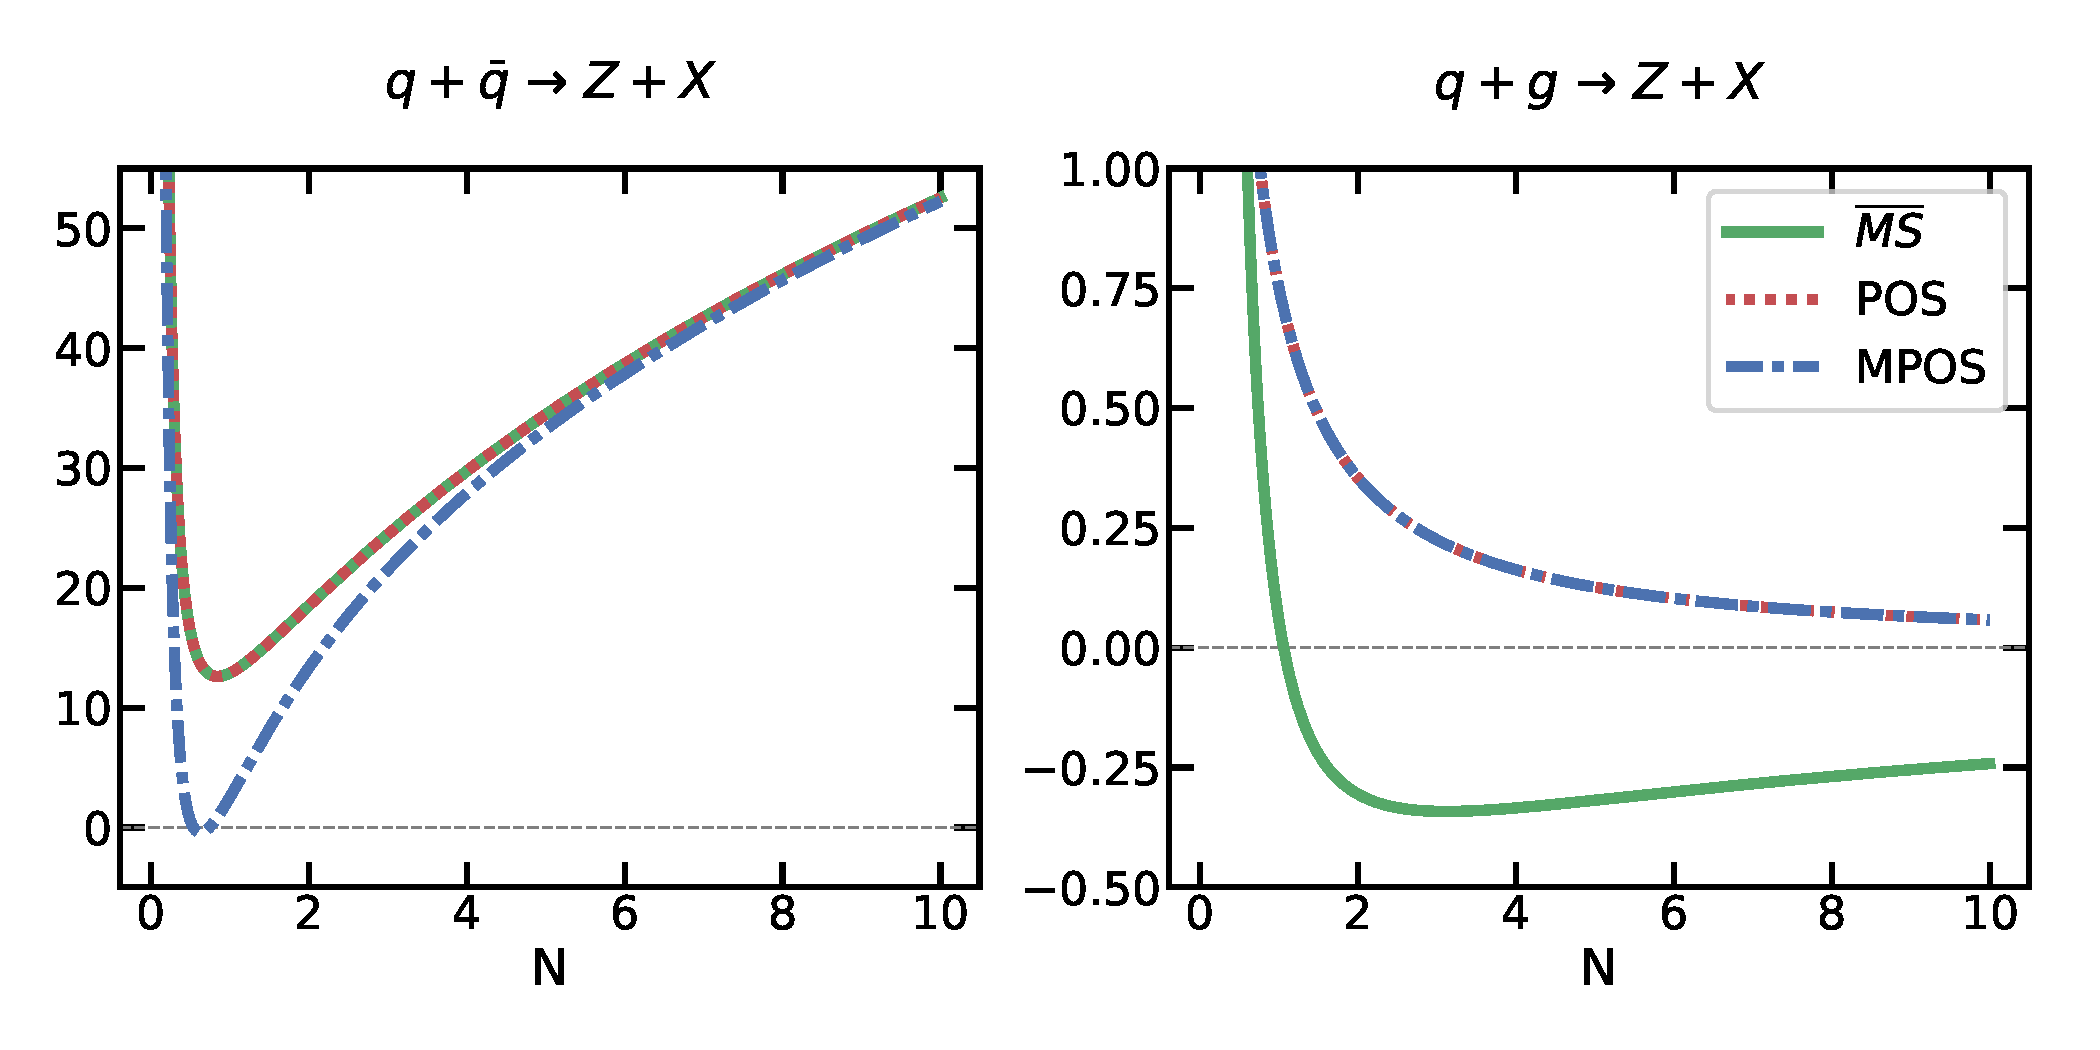
\includegraphics[width=0.8\linewidth]{ch-positivity/dy.pdf}
    \caption{\small Mellin-space NLO contributions to Drell--Yan coefficient
      functions. The quark (left) and gluon (right) coefficient
      functions, respectively  ${{{C^q}_q}^{(1)}}$ and  ${{{C^q}_g}^{(1)}}$, Eq.~(\ref{eq:hadfact}), are
      shown.
      Results are shown in the \msbar{}, POS and MPOS schemes. The POS
      scheme is defined in Eqs.~(\ref{eq:counthqq}-\ref{eq:counthqg})
      and (\ref{eq:counthgg}-\ref{eq:counthgq}), and the MPOS scheme
      in Eqs.~(\ref{eq:mposqq}-\ref{eq:mposgg}).
 ${{{C^q}_q}^{(1)}}$ \msbar{} and POS coincide, and the two curves
      correspond, from top to bottom, to \msbar{} and MPOS; for  
      ${{{C^q}_g}^{(1)}}$ POS and MPOS coincide and the two curves
      correspond, from top to bottom, to \msbar{} and POS. 
    \label{fig:dy} }
  \end{center}
\end{figure}
\subsubsection{The diagonal coefficient function}
\label{sec:diag}
We now turn to the diagonal coefficient function: in the \msbar{} scheme
it is given by
\begin{align}\label{eq:cq}
  C_q^{\mmsbar}(z)&=\delta(1-z)+ \frac{\alpha_s}{2\pi}
  {C^{(1)}_q}^{\mmsbar}(z)\\
    &=\delta(1-z) \left(1+\frac{\alpha_s}{2\pi} {\Delta^{(1)}_q}^{\mmsbar}\right)
  +\frac{\alpha_s}{2\pi}  {\overline{C_{q}}^{(1)}}^{\mmsbar}(z) \,,\label{eq:cqnodist}
\end{align}
where in the last step we have separated off the contribution to
$ {C^{(1)}_q}^{\mmsbar}(z)$ proportional to a Dirac $\delta$
(corresponding to a constant in Mellin space) so that
${\overline{C_{q}}^{(1)}}^{\mmsbar}(z)$ only contains  functions and
$+$ distributions.
The NLO diagonal
coefficient function is given by
\begin{align}
{C^{(1)}_q}^{\mmsbar}(z)&=
\lim_{\epsilon\to
  0^-}\left[C_{q}^{(1)}(z,Q^2,\epsilon) - \left(\frac{Q^2}{4\pi
      \mu^2}\right)^{-\epsilon} \left(-\frac 1
    {\epsilon}+\gamma_E\right) P_{qq}(z)\right]\label{eq:cqren}\\
&=\lim_{\epsilon\to0^-}\left[ {C_q^{(1)}}(z,Q^2,\epsilon)
    -\delta_{qq}^{\mmsbar}(z,Q^2,\epsilon)\right]\label{eq:renormq}\\
&= C_F\left[ \left(p_{qq}(z)
    \ln\left(\frac{1-z}{z}\right) \right)_+ - \frac {3}{2}\pDa{z} + 3
    + 2 z - 4 \delta(1-z)\right]\label{eq:cqnlo},
\end{align}
where 
$p_{qq}(z)$ is implicitly defined in terms of the quark-quark
splitting function $P_{qq}(z)$ as
\begin{equation}\label{eq:pqq}
  P_{qq}(z)= C_F\left(p_{qq}(z)\right)_+.
\end{equation}


The Mellin transform of $C^{(1)}_q(z)$ is shown in
Fig.~\ref{fig:dis}. It is clear that the coefficient function is
positive for all $N$: the slightly negative dip of the NLO term
in the $N\sim 1$
region is more than compensated by the much larger LO contribution,
which in $N$ space is a constant (at $\frac{2 \pi}{\alpha_s}$ on the
scale of Fig.~\ref{fig:dis}). 
As $N\to\infty$, where the NLO contribution diverges (and in
principle needs resummation) the growth is actually positive.

A comparison of Eq.~(\ref{eq:cqnlo}) with its off-diagonal counterpart,
Eq.~(\ref{eq:cgnlo}), immediately shows what is going on. In this
case too, the \msbar{} subtraction amounts to an over-subtraction, and
indeed the term proportional to $p_{qq}(z)$ in the coefficient
function Eq.~(\ref{eq:cqnlo}) has the same origin as the term
Eq.~(\ref{eq:logexp}), namely, the collinear singularity due to real
emission, in this case of a gluon from the incoming quark line. In
fact,  this is the contribution which is included in standard
leading-log threshold resummation. Amusingly, the further
(process-dependent)
term, proportional
to $\pDa{z}$, arises at the next-to-leading log level due to collinear
radiation from the outgoing quark line~\cite{Catani:1989ne}, and thus has
the same kinematic origin~\cite{Forte:2002ni}.
One may thus think of generally including these contributions in the
PDF by changing the collinear subtraction, as we did above: indeed
this is done in the Monte Carlo scheme of
Ref.~\cite{Jadach:2016acv}, which aims at including in PDFs
all contributions coming from soft radiation.


However, if the goal is ensure positivity, in the diagonal case
it is not necessary to
modify the \msbar{}  subtraction prescription. Indeed,
in this case over-subtraction actually leads to a more positive
coefficient function, due to the fact that the $P_{qq}$ splitting
function  is negative at large $z$, where it reduces to a $+$
distribution,
i.e., it leads to a negative answer
when folded with a positive test function. Of course, this follows from
baryon number conservation which requires the vanishing of the first
moment of the splitting function. It is in fact easy to check that the
\msbar{} coefficient function, Eq.~(\ref{eq:cq}), is positive for all
$z<1$. The  term proportional to a $\delta$ of course has a positive
coefficient in the perturbative regime, where it is dominated by the
LO term.

We conclude that in order to ensure positivity of the coefficient
function it is sufficient to modify the collinear subtraction only in the
off-diagonal channel. We therefore set
\begin{align}\label{eq:countq}
   {C_{q}^{(1)}}^{\textrm{DPOS}}(z)=  {C_{q}^{(1)}}^{\mmsbar}(z) \,.
\end{align}
Equations~(\ref{eq:count},\ref{eq:countq}) thus define the DPOS
factorization scheme in the quark channel, in terms of the \msbar{} scheme.
Note that the considerations underlying the construction of this
factorization scheme are based on the
structure of the collinear subtraction and the behavior of the
splitting functions, and are therefore process-independent.

In order to fully characterize the scheme it is necessary to also
consider gluon-induced processes. In Ref.~\cite{Altarelli:1998gn},
this was done by considering Higgs production in gluon fusion, with
one of the two gluons coming from a proton and the other being taken
as a pointlike probe. Equivalently, one might consider Higgs production in
photon-gluon fusion. However, the treatment of these
processes is essentially the same as that of hadronic processes, to
which we thus turn.


\subsection{Hadronic processes}
\label{sec:hadr}
For hadronic processes the basic factorization formula has the same structure
as Eq.~(\ref{eq:f2}), with the structure function replaced by a cross section
and the PDF replaced by a parton luminosity ${\cal L}_{ij}$: up to NLO
\begin{equation}
 \frac{1}{x} \sigma(x,Q^2)= \hat \sigma_0 \left[  {\cal L}_{ii}
   +\frac{\alpha_s}{2\pi}\left( {{C^i}_q}^{(1)} \otimes {\cal L}_{iq} +
 {{C^i}_g}^{(1)} \otimes {\cal L}_{ig}\right) \right],\label{eq:hadfact}
\end{equation}
where for simplicity we consider process for which at LO only one
partonic channel contributes, so
$i=q,g$ labels quark-induced processes (such as Drell--Yan) or
gluon-induced processes (such as Higgs production in gluon fusion),
$\hat{\sigma}_0$ is the LO partonic cross section and
the parton luminosity is 
\begin{equation}\label{eq:lumi}
 {\cal L}_{ij}= f_i\otimes f_j\,.
\end{equation}

We first discuss quark-induced processes: their treatment is very close to that
of DIS  presented in the previous section, so it is sufficient to highlight the
differences.
We then turn to gluon-induced processes, for which we repeat the analysis of
Sect.~\ref{sec:discf}.


\begin{figure}[t]
  \begin{center}
    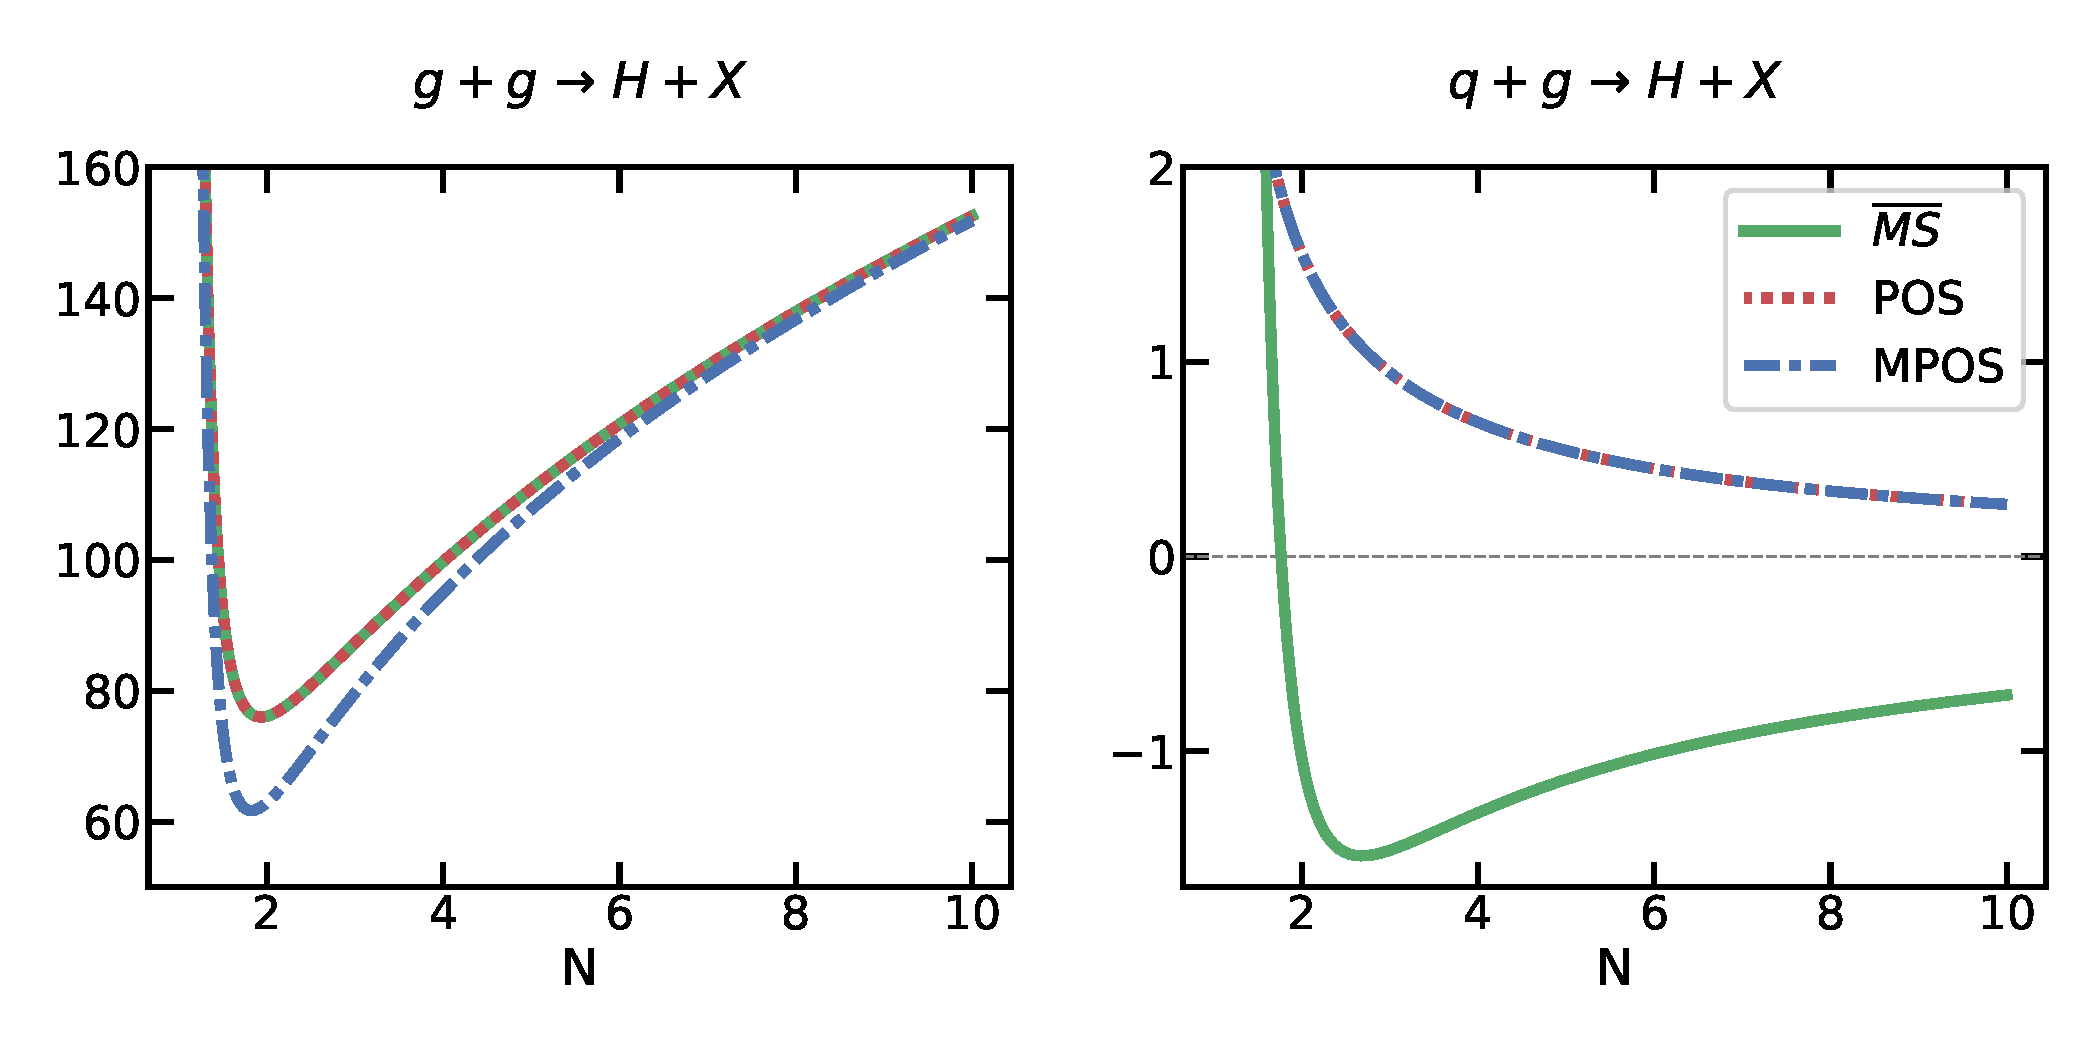
\includegraphics[width=0.8\linewidth]{ch-positivity/higgs.pdf}
    \caption{\small Same as Fig.~\ref{fig:dy}, but now for the Higgs
      coefficient functions  ${{{C^g}_g}^{(1)}}$ (left) and
      ${{{C^g}_q}^{(1)}}$ (right).
    \label{fig:higgs} }
  \end{center}
\end{figure}


\subsubsection{Quark-induced processes}
\label{sec:dy}
As a prototype of quark-induced process we consider Drell--Yan
production. The NLO coefficient functions (i.e.\ NLO partonic
cross sections normalized to the LO result) are given by 
\begin{align}\label{eq:dyq}
 {{C^q{}_q}^{(1)}}^{\mmsbar}(z)&= C_F\left[
 \left(\frac{4\pi^2}{3} - \frac 7 2\right)\delta(1-z) + 2
 \left(p_{qq}(z) \ln\left(\frac{(1-z)^2}{z}\right)
 \right)_+\right]\nonumber  \\
 &={\Delta_{qq}^{(1)}}^{\mmsbar}\delta(1-z) + 2 C_F \left(p_{qq}(z) \ln\left(\frac{(1-z)^2}{z}\right) \right)_+,\\
 \label{eq:dyg}
  {{C^q{}_g}^{(1)}}^{\mmsbar}(z)&= P_{qg}(z) \left[ \ln\left(\frac{(1-z)^2}{z}\right) - 1 \right]
  + C_F\left[\frac 3 2 -  \frac 3 2 z^2 + z\right].
\end{align}


Comparing the coefficient functions
Eq.~(\ref{eq:dyq}-\ref{eq:dyg}) to their DIS counterparts
Eqs.~(\ref{eq:cgren},\ref{eq:cqnlo}) shows that they have the same
structure, with a residual logarithmic contribution proportional to
the splitting function, due to over-subtraction. The only difference is
that the argument of the log is now $\frac{(1-z)^2}{z}$. This is again
recognized to be the upper limit of the transverse momentum integral,
and to coincide with the argument of the logs whose
renormalization-group improvement leads to threshold
resummation~\cite{Forte:2002ni}: indeed,
for a $2\to2$ process with a final state particle with mass $M^2$, and
$z=\frac{M^2}{s}$,
\begin{equation}\label{eq:ktmaxh}
\mu_h^2=  |k_T^{\textrm{max,\, had}}|^2=\frac{(s-Q^2)^2}{4s}=\frac{Q^2(1-z)^2}{4z}\,,
\end{equation}
where $ Q^2 = M^2 $.
The coefficient
functions, Eq.~(\ref{eq:dyq}-\ref{eq:dyg}), are displayed in
Fig.~\ref{fig:dy} in Mellin space; their qualitative features are the
same as those of the DIS coefficient functions.

Hence, just as in case of DIS, it is possible to define a positive
subtraction scheme, which we call POS, and which differs from \msbar{}
because in the off-diagonal quark-gluon channel the
subtraction is performed at the scale $\mu_h^2$,
Eq.~(\ref{eq:ktmaxh}). Just like for DIS, in the diagonal quark-quark
channel there is no need to modify the \msbar{} subtraction, which
actually makes the coefficient function more positive, so we define 
a POS factorization of the DY process according to
\begin{align}\label{eq:counthqq}
 {{C^q{}_q}^{(1)}}^{\textrm{POS}}(z) &=  {{C^q{}_q}^{(1)}}^{\mmsbar}(z) \,, \\
 {{C^q{}_g}^{(1)}}^{\textrm{POS}}(z) &=  {{C^q{}_g}^{(1)}}^{\mmsbar}(z) - K_{qg}^{\textrm{POS}} (z) \,,\\ \label{eq:counthqg}
  K_{qg}^{\textrm{POS}} (z) &=  P_{qg}(z)\left[\ln\left(\frac{(1-z)^2}{z}\right) - 1\right] \,.
\end{align}
The quark-gluon coefficient function can be read off
Eqs.~(\ref{eq:dyg},\ref{eq:counthqg}) and it is easy to check that it
is positive definite for all $0<z<1$.

Of course, a choice of factorization scheme must be
universal. Therefore, it is interesting to check what this choice
amounts to if adopted for DIS. Clearly, the
hadronic scale Eq.~(\ref{eq:ktmaxh}) is always lower than the DIS
scale Eq.~(\ref{eq:ktmaxh}): $\mu_h^2< \mu_D^2$. Hence, subtraction in the
DPOS scheme amounts to under-subtraction, and if adopted for DIS
coefficient function it leads to a DIS coefficient function
${C^{(1)}_{g}}^{\textrm{POS}}(z)$ which is actually more positive than that
in the DPOS scheme. This is seen in Fig.~\ref{fig:dis} (right), where 
${C^{(1)}_{g}}(z)$ is shown in the \msbar{}, DPOS and POS schemes.

\subsubsection{Gluon-induced processes}
\label{sec:higgs}
In order to fix completely the factorization scheme we turn to
gluon-induced hadronic processes. We choose Higgs production in gluon
fusion (in the infinite top mass limit) as a prototype, and we repeat the  analysis of
Sect.~\ref{sec:offdiag}, but now for the quark coefficient function
${{{C^g}_q}^{(1)}}$. The regularized, unsubtracted expression is (see
e.g.~\cite{Maltoni:2018dar}) 
\begin{equation}\label{eq:cgqeps}
{C^g{}_q}^{(1)}(z,Q^2,\epsilon) =
  \frac{ \Gamma(-\epsilon)
  \left(\frac{\mu_h^2}{\pi\mu^2}\right)^{-\epsilon} (1-\epsilon) \left[P_{gq}(z) - C_F \frac{(1+z)^2}{2z} \epsilon \right]}{16\pi (2 - 2\epsilon) \Gamma (3 - 2 \epsilon)}\,,
\end{equation}
where $\mu_h^2$ is given by Eq.~(\ref{eq:ktmaxh}), with $Q^2=M_H^2$,
the Higgs square mass.
Performing  \msbar{} subtraction in the usual way we get
\begin{align}\label{eq:cgqren}
{  {C^g{}_q}^{(1)}}^{\mmsbar}(z) &= \lim_{\epsilon\to
  0^-}\left[{{C^{g}}_q}^{(1)}(z,Q^2,\epsilon) - \left(\frac{Q^2}{4\pi
      \mu^2}\right)^{-\epsilon} \left(-\frac 1
    {\epsilon}+\gamma_E\right) P_{gq}(z)\right]\\
&= P_{gq}(z)\left[\ln\left(\frac{(1-z)^2}{z}\right) - 1 \right]  + C_F \frac{(1+z)^2}{2z} 
 \,.\label{eq:cgqnlo}
\end{align}

Again, we encounter the same situation that we have seen in the quark
channel for DIS, Eqs.~(\ref{eq:cgeps},\ref{eq:cgren}): the collinear
log has a scale set by the upper limit of the transverse momentum
integration, now the hadronic $\mu_h^2$, Eq.~(\ref{eq:ktmaxh}), but the
\msbar{} subtraction is performed at the scale $Q^2$, which at large $z$
is higher, thus leading to over-subtraction. Indeed, the Mellin-space
\msbar{} coefficient function  ${{{C^g}_q}^{(1)}}$, shown in
Fig.~\ref{fig:higgs}, is seen to be negative at large $N$.

As in the quark sector, the problem is fixed by performing the
collinear subtraction at the physical scale $\mu_h^2$. Note that
also in this case, as for the DIS quark-gluon channel,
there is an issue with the sum over gluon polarizations: indeed,
because the LO process is in the gluon-gluon channel, even the NLO
quark-gluon channel has a gluon in the initial state, leading
to a factor  $1-\epsilon$ in the 
denominator of Eq.~(\ref{eq:cgqeps}), which must be accounted for in
order to avoid over-subtraction.
Hence, we define the POS scheme coefficient function as
\begin{align}\label{eq:cqrenposh}
  {{C^g{}_q}^{(1)}}^{\textrm{POS}} (z)  &= \lim_{\epsilon\to0^-}
  \left[  {C^g{}_q}^{(1)}(z,Q^2,\epsilon) - \frac{1}{1-\epsilon}\left(\frac{\mu_h^2}{\pi\mu^2}\right)^{-\epsilon} \left(-\frac 1
    {\epsilon}+\gamma_E\right) P_{qg}(z)\right]\\ \label{eq:cqrenposh1}
    &=C_F \frac{(1+z)^2}{2z} \, ,
\end{align}
with $\mu_h^2$ given by Eq.~(\ref{eq:ktmaxh}).
The coefficient function is clearly positive. Its Mellin transform is
also shown in Fig.~\ref{fig:higgs}.

We finally examine the gluon-gluon NLO coefficient function:
\begin{align}\label{eq:higgsg}
\hspace*{-30pt}  {{C^g{}_g}^{(1)}}^{\mmsbar} (z) &=C_A\left[ 2\frac 1 z \left(z p_{gg}(z) \ln\left(\frac{(1-z)^2}{z}\right) \right)_++
    \left(\frac{473}{36} + \frac{4\pi^2}{3}\right)\delta(1-z) -
    \frac{11}{3}\frac{(1-z)^3}{z}\right]\nonumber\\
&={\Delta^{(1)}_{gg}}^{\mmsbar}\delta(1-z)+ C_A\left[ 2\frac 1 z \left(z p_{gg}(z) \ln\left(\frac{(1-z)^2}{z}\right) \right)_+-
    \frac{11}{3}\frac{(1-z)^3}{z}\right] \,,
\end{align}
where, in analogy to Eq.~(\ref{eq:pqq}), $p_{gg}(x)$ is implicitly
defined by
\begin{equation}\label{eq:pgg}
  P_{gg}(z)= C_A\frac 1 z \left(z p_{gg}(z)\right)_+ - \frac{n_f}{3} \delta(1-z).
\end{equation}
As in the diagonal quark channel, the \msbar{} subtraction is now
multiplied by a splitting function which is negative at large $z$, for
the same physical reason. It therefore leads to a coefficient function
which is positive, as seen by inspecting Eq.~(\ref{eq:higgsg}) and
shown in Fig.~\ref{fig:higgs} (left), so no further scheme change is needed.

Therefore we get
\begin{align}\label{eq:counthgg}
 {{C^g{}_g}^{(1)}}^{\textrm{POS}}(z) &=  {{C^g{}_g}^{(1)}}^{\mmsbar}(z) \,, \\
 {{C^g{}_q}^{(1)}}^{\textrm{POS}}(z) &=  {{C^q{}_g}^{(1)}}^{\mmsbar}(z) - K_{gq}^{\textrm{POS}} (z) \,,\\ \label{eq:counthgq}
  K_{gq}^{\textrm{POS}} (z) &=  P_{gq}(z)\left[\ln\left(\frac{(1-z)^2}{z}\right)
    - 1\right].
\end{align}

Equations~(\ref{eq:counthqq}-\ref{eq:counthqg}) and (\ref{eq:counthgg}-\ref{eq:counthgq}) 
fully define the POS subtraction. We shall see in the next section
that they define a positive factorization scheme. Indeed, in the
construction presented in this section we have not made use of the
detailed from of the partonic cross section, but rather just of the
collinear counterterms, expressed in terms of universal splitting
functions. Hence, these counterterms, when used in
Eq.~(\ref{eq:pertz})  define a universal renormalization scheme
Eq.~(\ref{eq:pdffac}) for PDFs, without spoiling PDF universality.

